\section{Hardwaretests}\label{text:Entwicklung-der-GFA:Hardwaretests}

Im Rahmen der Entwicklungsprozesse einer Gleisfreimeldeanlage kommt den Hardwaretests eine ebenso signifikante wie den Softwareprüfungen zustehende Bedeutung zu. Diese Tests dienen der Verifizierung der Funktionsfähigkeit und der Leistungsfähigkeit der physischen Komponenten unter realitätsnahen Einsatzbedingungen. Im nachfolgenden Abschnitt wird eine umfassende Darstellung der für die Sicherstellung der Zuverlässigkeit und Effizienz der Gleisfreimeldeanlage unerlässlichen Hardwaretests vorgenommen. Es werden die angewendeten Methodiken, Instrumente und Verfahrensweisen erörtert, welche essentiell sind, um die Funktionalität, Beständigkeit und die Interoperabilität der Hardwarekomponenten zu evaluieren. Dies geschieht mit dem Ziel, die Einhaltung der hohen Sicherheits- und Leistungsstandards im Eisenbahnwesen zu gewährleisten.

\subsection{Aufbau}

Die Hardwaretests der Gleisfreimeldeanlage kombinieren in erster Linie die Reed-Kontakte mit der Software und überprüfen deren Funktionalität. Um schnell verschiedene Umstände testen zu können und die Fehlersuche zu minimieren wurden diese Tests auf einem Steckbrett durchgeführt. Das Steckbrett ist in \autoref{fig:HWTest-bb} dargestellt.
\begin{figure}[H]
    \centering
    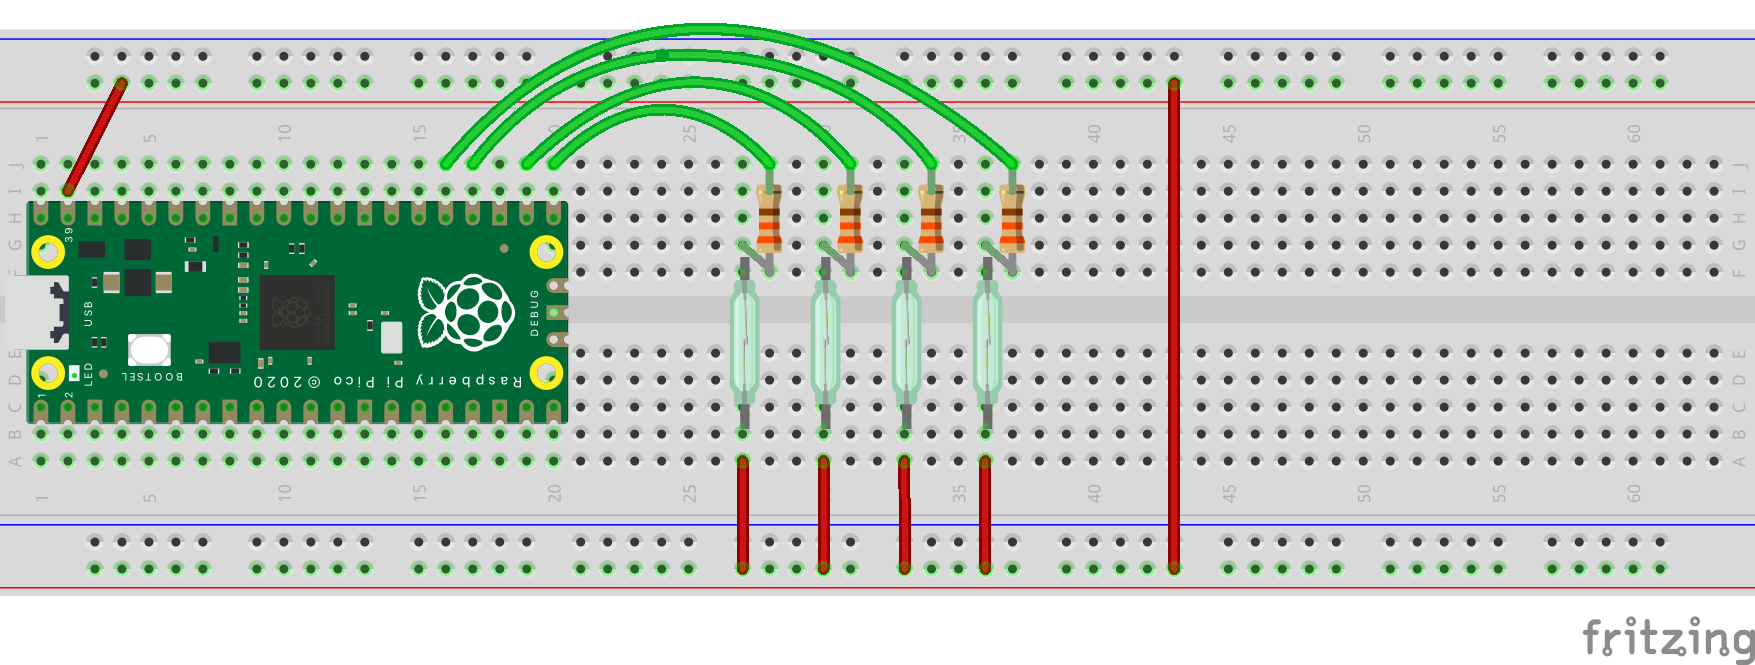
\includegraphics[width=0.7\textwidth]{Assets/Images/4-Entwicklung-der-GFA/Reed-Test_bb.png}
    \caption{Aufbau der Hardwaretests auf einem Steckbrett}
    \label{fig:HWTest-bb}
\end{figure}

Um die Zustände der Software zu visualisieren, wurden zusätzlich LEDs auf dem Steckbrett verbaut. Diese LEDs zeigen sowohl den aktuellen Zählerstand des simulierten Streckenabschnitts, als auch den aktuellen Error-Code in 3-Bit Darstellung an. Die Schaltung hinter den LEDs ist trivial und wird daher nicht weiter beschrieben.

\subsection{Testszenarien}

Die Testszenarien für die Hardwaretests sind in erster Linie auf die Software zurück zu führen. Hierbei verliefen die ersten Tests zunächsts zufallsbasiert. Nach und nach wurden aber auch spezifische Testszenarien entwickelt, umd die Funktionalität der Software zu überprüfen. Diese Tests sind kausal zu den Softwaretests welche in \autoref{text:Entwicklung-der-GFA:Softwaretests:Tests-für-Geraden} \nameref{text:Entwicklung-der-GFA:Softwaretests:Tests-für-Geraden} beschrieben sind. 
